\documentclass[12pt, leqno]{article} %% use to set typesize
\usepackage{fancyhdr}
\usepackage[letterpaper=true,colorlinks=true,linkcolor=black]{hyperref}

\usepackage{amsfonts}
\usepackage{amsmath,amssymb,amsthm}
\usepackage{color}
\usepackage{tikz}
\usepackage{pgfplots}
\usepackage{listings}
%\usepackage{courier}
%\usepackage[utf8]{inputenc}
%\usepackage[russian]{babel}

\lstdefinelanguage{Julia}%
  {morekeywords={abstract,break,case,catch,const,continue,do,else,elseif,%
      end,export,false,for,function,immutable,import,importall,if,in,%
      macro,module,otherwise,quote,return,switch,true,try,type,typealias,%
      using,while},%
   sensitive=true,%
   alsoother={$},%
   morecomment=[l]\#,%
   morecomment=[n]{\#=}{=\#},%
   morestring=[s]{"}{"},%
   morestring=[m]{'}{'},%
}[keywords,comments,strings]%

\lstset{
  numbers=left,
  basicstyle=\ttfamily\footnotesize,
  numberstyle=\tiny\color{gray},
  stepnumber=1,
  numbersep=10pt,
}

\newcommand{\iu}{\ensuremath{\mathrm{i}}}
\newcommand{\bbR}{\mathbb{R}}
\newcommand{\bbC}{\mathbb{C}}
\newcommand{\calV}{\mathcal{V}}
\newcommand{\calE}{\mathcal{E}}
\newcommand{\calG}{\mathcal{G}}
\newcommand{\calW}{\mathcal{W}}
\newcommand{\calP}{\mathcal{P}}
\newcommand{\macheps}{\epsilon_{\mathrm{mach}}}
\newcommand{\matlab}{\textsc{Matlab}}
\newcommand{\uQ}{\underline{Q}}
\newcommand{\uR}{\underline{R}}

\newcommand{\ddiag}{\operatorname{diag}}
\newcommand{\fl}{\operatorname{fl}}
\newcommand{\nnz}{\operatorname{nnz}}
\newcommand{\tr}{\operatorname{tr}}
\renewcommand{\vec}{\operatorname{vec}}

\newcommand{\vertiii}[1]{{\left\vert\kern-0.25ex\left\vert\kern-0.25ex\left\vert #1
    \right\vert\kern-0.25ex\right\vert\kern-0.25ex\right\vert}}
\newcommand{\ip}[2]{\langle #1, #2 \rangle}
\newcommand{\ipx}[2]{\left\langle #1, #2 \right\rangle}
\newcommand{\order}[1]{O( #1 )}

\newcommand{\kron}{\otimes}


\newcommand{\hdr}[1]{
  \pagestyle{fancy}
  \lhead{Bindel, Fall 2022}
  \rhead{Matrix Computations}
  \fancyfoot{}
  \begin{center}
    {\large{\bf #1}}
  \end{center}
  \lstset{language=Julia,columns=flexible}  
}


\begin{document}

\hdr{2022-09-15}

\section{Band and skyline solvers}

In this lecture, we will consider various types of sparse direct
factorization methods.  We'll focus throughout on Cholesky, simply to
avoid the awkwardness associated with pivoting.  We begin with the
case of band matrices.

The {\em bandwidth} $b$ of a matrix is the smallest non-negative
integer $b$ such that $a_{ij} = 0$ for $|i-j| > b$.  Hence, diagonal
matrices have bandwidth 1, bidiagonal and tridiagonal matrices have
bandwidth 2, and so forth.  In the nonsymmetric case, we may
distinguish between the upper and the lower bandwidth.

For symmetric positive definite matrices of bandwidth $b$, the
Cholesky factors also have bandwidth $b$.  To see why, consider one
step of Cholesky factorization for a pentadiagonal matrix (bandwidth
$b = 2$):
\[
A = \begin{bmatrix}
  \times & \times & \times \\
  \times & \times & \times & \times \\
  \times & \times & \times & \times & \times \\
  & \times & \times & \times & \times & \times \\  
  & & \times & \times & \times & \times & \times \\
  & & & \ddots & \ddots & \ddots & \ddots & \ddots \\
  & & & & \times & \times & \times & \times & \times \\
  & & & & & \times & \times & \times & \times \\
  & & & & & & \times & \times & \times \\
  \end{bmatrix}
\]
The first step of Cholesky factorization takes the square root of the
$(1,1)$ element, scales the first row, and (conceptually) zeros out
the subdiagonal entries of the first column.  If we mark the modified
entries with stars, we have
\[
  \begin{bmatrix}
  * & * & * \\
  0 & \times & \times & \times \\
  0 & \times & \times & \times & \times \\
  & \times & \times & \times & \times & \times \\  
  & & \times & \times & \times & \times & \times \\
  & & & \ddots & \ddots & \ddots & \ddots & \ddots \\
  & & & & \times & \times & \times & \times & \times \\
  & & & & & \times & \times & \times & \times \\
  & & & & & & \times & \times & \times \\
  \end{bmatrix}.
\]
The entries multiplied in the Schur complement update are those in the
$(2:b) \times (2:b)$ block
\[
  \begin{bmatrix}
  * & * & * \\
  0 & * & * & \times \\
  0 & * & * & \times & \times \\
  & \times & \times & \times & \times & \times \\  
  & & \times & \times & \times & \times & \times \\
  & & & \ddots & \ddots & \ddots & \ddots & \ddots \\
  & & & & \times & \times & \times & \times & \times \\
  & & & & & \times & \times & \times & \times \\
  & & & & & & \times & \times & \times \\
  \end{bmatrix}.
\]
We now observe that the Schur complement continues to have bandwidth
$b$, and so this same pattern will repeat throughout the
factorization.

Nonsymmetric band solvers may involve pivoting, but even then the band
structure cannot increase by very much.  In each case, by using
compact representations of band matrices, we can compute an LU or
Cholesky factorization using $O(nb^2)$ time and $O(nb)$ space.  And,
once the factorization is computed, forward and backward substitution
steps then take $O(nb)$ time as well.

A generalization of band solvers is the {\em profile} or {\em skyline}
solver.  In a row-oriented skyline format in the case where we are tracking the
lower triangle, we keep each row of the lower triangle consecutively
in memory, and separately keep the index of the start of each row.
In each column, the first nonzero defines the start of the profile.
With this convention, all fill-in with a band solver is again confined
to the profile.

\section{General sparse direct methods}

Suppose $A$ is a general sparse matrix, and $PA = LU$.  Will $L$ and $U$ also
be sparse?  The answer depends in a somewhat complicated way on the
structure of the graph associated with the matrix $A$, the pivot
order, and the order in which variables are eliminated.  Except in
very special circumstances, there will generally be more nonzeros in
$L$ and $U$ than there are in $A$; these extra nonzeros are referred
to as {\em fill}.  There are two standard ideas for minimizing fill:
\begin{enumerate}
\item
  Apply a {\em fill-reducing ordering} to the variables; that is,
  use a factorization
  \[
    PAQ = LU,
  \]
  where $Q$ is a column permutation chosen to approximately minimize
  the fill in $L$ and $U$, and $P$ is the row permutation used for
  stability.

  The problem of finding an elimination order that minimizes fill is
  NP-hard, so it is hard to say that any ordering strategy is really
  optimal.  But there is canned software for some heuristic orderings
  that tend to work well in practice.  From a practical perspective,
  then, the important thing is to remember that a fill-reducing
  elimination order tends to be critical to using sparse Gaussian
  elimination in practice.
\item
  Relax the standard partial pivoting condition, choosing the row
  permutation $P$ to balance the desire for numerical stability
  against the desire to minimize fill.
\end{enumerate}

For the rest of this lecture, we will consider the simplified case of
{\em structurally} symmetric matrices and factorization without
pivoting (which you know from last week's guest lectures is stable for
diagonally dominant systems and positive definite systems).

\section{Sparse matrices, graphs, and tree elimination}

Consider the following illustrative example of how factoring a sparse
matrix can lead to more or less dense factors depending on the order
of elimination.  Putting in $\times$ to indicate a nonzero element, we
have
\[
  \begin{bmatrix}
    \times & \times & \times & \times & \times \\
    \times & \times &        &        &        \\
    \times &        & \times &        &        \\
    \times &        &        & \times &        \\
    \times &        &        &        & \times
  \end{bmatrix} =
  \begin{bmatrix}
    \times &        &        &        &        \\
    \times & \times &        &        &        \\
    \times & \times & \times &        &        \\
    \times & \times & \times & \times &        \\
    \times & \times & \times & \times & \times
  \end{bmatrix}
  \begin{bmatrix}
    \times & \times & \times & \times & \times \\
           & \times & \times & \times & \times \\
           &        & \times & \times & \times \\
           &        &        & \times & \times \\
           &        &        &        & \times
  \end{bmatrix}.
\]
That is, $L$ and $U$ have many more nonzeros than $A$.
These nonzero locations that appear in $L$ and $U$ and not in $A$
are called {\em fill-in}.  On the other hand, if we cyclically
permute the rows and columns of $A$, we have
\[
  \begin{bmatrix}
    \times &        &        &        & \times \\
           & \times &        &        & \times \\
           &        & \times &        & \times \\
           &        &        & \times & \times \\
    \times & \times & \times & \times & \times
  \end{bmatrix} =
  \begin{bmatrix}
    \times &        &        &        & \\
           & \times &        &        & \\
           &        & \times &        & \\
           &        &        & \times & \\
    \times & \times & \times & \times & \times
  \end{bmatrix}
  \begin{bmatrix}
    \times &        &        &        & \times \\
           & \times &        &        & \times \\
           &        & \times &        & \times \\
           &        &        & \times & \times \\
           &        &        &        & \times
  \end{bmatrix}.
\]
That is, the factorization of $PAP^T$ has {\em no} fill-in.

A sparse matrix $A$ can be viewed as an {\em adjacency matrices}
for an associated graphs: make one node for each row,
and connect node $i$ to node $j$ if $A_{ij} \neq 0$.  The graphs
for the two ``arrow'' matrices above are:
%\begin{center}
%\input{lec16fig1.pdf_t}
%\end{center}
\begin{center}
  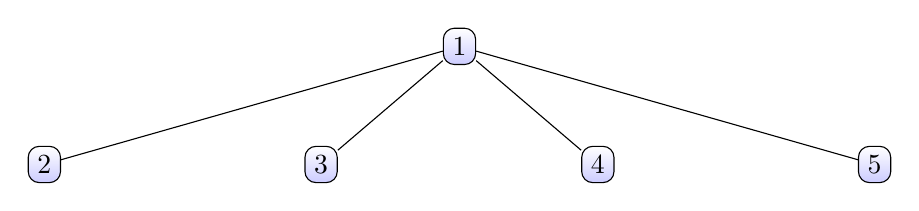
\begin{tikzpicture}[sibling distance=10em,
    every node/.style = {shape=rectangle, rounded corners,
    draw, align=center, top color=white, bottom color=blue!20}]
    \node {1}
      child { node {2} }
      child { node {3} }
      child { node {4} }
      child { node {5} };
  \end{tikzpicture}
  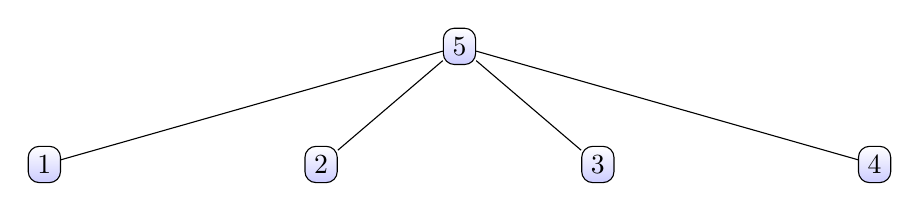
\begin{tikzpicture}[sibling distance=10em,
    every node/.style = {shape=rectangle, rounded corners,
    draw, align=center, top color=white, bottom color=blue!20}]
    \node {5}
      child { node {1} }
      child { node {2} }
      child { node {3} }
      child { node {4} };
  \end{tikzpicture}
\end{center}

These graphs of both our example matrices are {\em trees}, and they
differ only in how the nodes are labeled.  In the original matrix, the
root node is assigned the first label; in the second matrix, the root
node is labeled after all the children.  Clearly, the latter label
order is superior for Gaussian elimination.  This turns out to be a
general fact: if the graph for a (structurally symmetric) sparse
matrix $S$ is a tree, and if the labels are ordered so that each node
appears after any children it may have, then there is no fill-in: that
is, $L$ and $U$ have nonzeros only where $S$ has nonzeros.

Why should we have no fill when factoring a matrix for a tree ordered
from the leaves up?  To answer this, we think about what happens in the
first step of Gaussian elimination.  Our original matrix has the form
\[
  S = \begin{bmatrix} \alpha & w^T \\ v & S_{22} \end{bmatrix}
\]
The first row of $U$ is identical to the first row of $S$,
and the first column of $L$ has the same nonzero structure
as the first column of $A$, so we are fine there.
The only question is about the nonzero structure of the Schur
complement $S_{22}-vw^T/\alpha$.  Note that the update $vw^T/\alpha$
has nonzeros only where $v_i$ and $w_j$ are both nonzero --- that is,
only when nodes $i$ and $j$ are both connected to node $1$.  But node
1 is a leaf node; the only thing it connects to is its parent!  So if
$p$ is the index of the parent of node 1 in the tree, then we only
change the $(p,p)$ entry of the trailing submatrix during the update
--- and we assume that entry is already nonzero.  Thus, the graph
associated with the Schur complement is the same as the graph of the
original matrix, but with one leaf trimmed off.

\section{Nested dissection}

Tree-structured matrices are marvelous because we can do everything in
$O(n)$ time: we process the tree from the leaves to the root in order
to compute $L$ and $U$, then recurse from the root to the leaves in
order to do back substitution with $U$, and then go back from the
leaves to the root in order to do forward substitution with $L$.
Sadly, many of the graphs we encounter in practice do not look like trees.
However, we can often profitably think of clustering nodes so that we get
a {\em block} structure associated with a tree.

For illustrative purposes, let us consider Gaussian elimination on a
matrix whose graph is a regular $n \times n$ mesh.  Such a matrix
might arise, for example, if we were solving Poisson's equation using
a standard five-point stencil to discretize the Laplacian operator.
We then think of cutting the mesh in half by removing a set of
separator nodes, cutting the halves in half, and so forth.  This
yields a block structure of a tree consisting of a root (the separator
nodes) and two children (the blocks on either side of the separator).
We can now dissect each of the sub-blocks with a smaller separator,
and continue on in this fashion until we have cut the mesh into blocks
containing only a few nodes each.  Figure~\ref{fig1} illustrates the
first two steps in this process of {\em nested dissection}.

\begin{figure}
\begin{center}
\input{fig/ndfig.pdf_t}
\[
  S =
  \begin{bmatrix}
    S_{AA} &        & {\color[rgb]{0,0,1}S_{AC}} &      &        &       & {\color[rgb]{1,0,0}S_{AG}} \\
           & S_{BB} & {\color[rgb]{0,0,1}S_{BC}} &      &        &       & {\color[rgb]{1,0,0}S_{BG}} \\
    {\color[rgb]{0,0,1}S_{CA}} & {\color[rgb]{0,0,1}S_{CB}} & {\color[rgb]{0,0,1} S_{CC}} &       &        &       & {\color[rgb]{1,0,0}S_{CG}} \\
           &       &       & S_{DD} &        & {\color[rgb]{0,0,1}S_{DF}} & {\color[rgb]{1,0,0}S_{DG}} \\
           &       &       &       & S_{EE} & {\color[rgb]{0,0,1}S_{EF}} & {\color[rgb]{1,0,0}S_{EG}} \\
           &       &       & {\color[rgb]{0,0,1}S_{FD}} & {\color[rgb]{0,0,1}S_{FE}} & {\color[rgb]{0,0,1}S_{FF}} & {\color[rgb]{1,0,0}S_{FG}} \\
    {\color[rgb]{1,0,0}S_{GA}} & {\color[rgb]{1,0,0}S_{GB}} & {\color[rgb]{1,0,0}S_{GC}} & {\color[rgb]{1,0,0}S_{GD}} & {\color[rgb]{1,0,0}S_{GE}} & {\color[rgb]{1,0,0}S_{GF}} & {\color[rgb]{1,0,0}S_{GG}}
  \end{bmatrix}
\]
\end{center}
\caption{Nested dissection on a square mesh.  We first cut the graph in half
         with the red separator $G$, then further dissect the halves with the
         blue separators $C$ and $F$.  Nodes in $A$, $B$, $D$, and $F$ are only
         connected through these separator nodes, which is reflected in the
         sparsity pattern of the adjacency matrix $S$ when it is ordered so that
         separators appear after the things they separate.}
\label{fig1}
\end{figure}

We can get a lower bound on the cost of the factorization by figuring
out the cost of factoring the Schur complement associated with $G$,
$C$, $F$, etc.  After we eliminate everything except the nodes
associated with $G$, we pay about $2n^3/3$ flops to factor the
remaining (dense) $n$-by-$n$ Schur complement matrix $G$.  Similarly,
we pay about $2(n/2)^3/3$ time to factor the dense $(n/2)$-by-$(n/2)$
complements associated with the separators $C$ and $F$.  Eliminating
all four separators then costs a total of $\approx 10n^3/12$ flops.
Now, think of applying nested dissection to blocks $A$, $B$, $D$, and
$E$; eliminating the Shur complements associated with separators
inside each of these blocks will take about $5(n/2)^3/6$ flops; all
four together cost a total of $4 ( 5(n/2)^3/6 )= (1/2)
(5n^3/6)$ flops to factor.  If we keep recursing, we find that the
cost of factoring Schur complements associated with all the separators
looks like
\[
  \frac{5}{6} n^3 \left( 1 + \frac{1}{2} + \frac{1}{4} + \ldots \right)
  \approx \frac{5}{3}n^3.
\]
It turns out that forming each Schur complement is asymptotically not
more expensive than eliminating it, so that the overall cost of doing
nested dissection on an $n \times n$ mesh with $N = n^2$ unknown is also
$O(n^3) = O(N^{1.5})$.  It also turns out that the fill-in is
$O(N \log N)$\footnote{
  The explanation of why is not so hard, at least for regular 2D meshes,
  but it requires more drawing than I feel like at the moment.  The paper
  ``Nested Dissection of a Regular Finite Element Mesh'' by Alan George
  (SIAM J. Numer. Anal. 10(2), April 1973) gives a fairly readable explanation
  for the curious.
}.

Now think about doing the same thing with a three-dimensional mesh.
In this case, the top-level separators for an $n \times n \times n$ mesh
with $N = n^3$ unknowns would involve $n^2$ unknowns, and we would take
$O(n^6) = O(N^2)$ time to do the elimination, and $O(N^{4/3})$ fill.
This relatively poor scaling explains why sparse direct methods are attractive
for solving 2D PDEs, but are less popular for 3D problems.

\section{Sparse solvers in practice}

Well-tuned sparse elimination codes do not have quite the flop rate of
dense linear algebra, but they are nonetheless often extremely fast.
In order to get this speed, though, quite a bit of engineering is
needed.  In the remainder of these notes, we sketch some of these
engineering aspects -- but we do so largely to convince you that you
are better off using someone else's sparse solver code than rolling
your own!  If you want all the gory details, I highly recommend Tim
Davis's book {\em Direct Methods for Sparse Linear Systems} (a SIAM
publication that is available in electronic form through the Cornell
library).

\subsection{Symbolic factorization}

Typical sparse Cholesky codes involve two stages:
a {\em symbolic factorization} stage in which the nonzero structure
of the factors is computed, and a {\em numerical factorization} stage
in which we fill in that nonzero structure with actual numbers.  One
advantage of this two-stage approach is that we can re-use the
symbolic factorization when we are faced with a series of matrices
that all have the same nonzero structure.  This happens frequently in
nonlinear PDE solvers, for example: the Jacobian of the discretized
problem changes at each solver step (or each time step), but the
nonzero structure often remains fixed.

\subsection{(Approximate) minimum degree ordering}

When we have a clear geometry, nested dissection ordering can be very
useful.  Indeed, nested dissection is useful in some cases even when
we have ``lost'' the geometry -- we can use spectral methods (which we
will describe later in the course) to find small separators in the
graph.  But in some cases, there is no obvious geometry, or we don't
want to pay the cost of computing a nested dissection ordering.  In
this case, a frequent alternative approach is a {\em minimum degree
  ordering}.  The idea of minimum degree ordering is to search the
Schur complement graph for the node with smallest degree, since the
fill on eliminating that variable is bounded by the square of the
degree.  Then we eliminate the vertex, update the degrees of the
neighbors, and repeat.  Unfortunately, this is expensive to implement
in the way described here -- better variants (using quotient graphs)
are more frequently used in practice.

\subsection{Cache locality}

In order to get good use of level 3 BLAS, sparse direct factorization
routines often identify dense ``supernodal'' structure in the factor.
We have already seen one case where this happens in our discussion of
nested dissection: we get dense blocks arising from separator Schur
complements.  The main alternative to supernodal solvers is the family
of {\em multifrontal} solvers, which also are able to take advantage
of level 3 BLAS.

\subsection{Elimination trees and parallelism}

An {\em elimination tree} in Gaussian elimination (or Cholesky) is a
tree on $n$ nodes, one per column or variable.  We say $j$ is a
descendant of $k$ if eliminating $j$ updates node $k$.  The nice thing
about this structure is that it identifies opportunities for
parallelism: disjoint subtrees of the elimination tree do not directly
interact, and can be eliminated in parallel in the numerical
factorization.

\end{document}
